\chapter{A LUZ COMO MATERIAL}

De acordo com \citeonline[p. 18]{vega} os artistas, em diferentes épocas, se viram inspirados e cativados pela luz, tanto a natural quanto a artificial, e tentaram capturar seu mistério e sua natureza mágica em suas criações. Alguns em particular, como Caravaggio, Vermeer e Monet, buscaram retratar, quase como uma obsessão, a luz e seus efeitos no mundo ao seu redor e, mais recentemente, os artistas contemporâneos vem se utilizando da luz como matéria-prima, realizando manipulações em três dimensões para projetar suas dimensões infinitas. 

Para entendermos como se deu, na arte, o uso da luz como material, precisamos compreender o processo de rompimento do pensamento clássico, a mímese, para o romântico, a \textit{poiesis}, afirma \citeonline[p. 74]{henno}. Portanto, ainda que o objeto dessa pesquisa seja a luz como meio, faz-se necessário traçar um breve panorama histórico de como a mesma se manifesta ao longo da história da arte. Além disso, dedicaremos parte deste capítulo a explorar obras de artistas contemporênos que trabalham a luz como material em um contexto de interatividade. E, por fim, vamos buscar compreender o cenário e a importância do cubo preto para exibição desse tipo de obra.


\section{A LUZ NA HISTÓRIA DA ARTE}

De acordo com  \citeonline[p.73]{henno} desde os primórdios da humanidade, quando o homem descobria o fogo, a luz sempre desencadeou fascínio. Esse deslumbramento se manifesta de maneiras distintas ao longo da história da arte. \citeonline{muga} afirma que "a experiência da luz atravessou três paradigmas ao longo da história: o paradigma da luz atributo - a luz venerada; o paradigma da luz efeito - a luz domesticada; e o paradigma da luz causa - a luz instrumentalizada".

Referindo-se à luz venerada, \citeonline{muga} observa que ela é percebida essencialmente como um atributo dos objetos, uma propriedade que lhes é inerente e não como um resultado da incidência luminosa. De acordo com \apudonline{arnheim}{muga} até o renascimento a luz era usada basicamente como um meio de modelar o volume e não enquanto efeito da iluminação. Nesse contexto, o mundo é claro, os objetos são por si só luminosos e as sombras são aplicadas para sugerir rotundidade. Destaca também que, na arte religiosa, os fundos dourados, as auréolas e as línguas de fogo aparecem como atributos brilhantes, representações simbólicas da divindade e não como reflexo da luz. Podemos ver um exemplo destes atributos na figura \ref{fig:giotto_lamentacao} que mostra a obra \textit{A lamentação} de Giotto de Bondone.

\begin{figure}[H]
  \begin{center}
    \caption{\textit{A lamentação} (1305), Giotto de Bondone}
    \vspace*{0,2cm}
    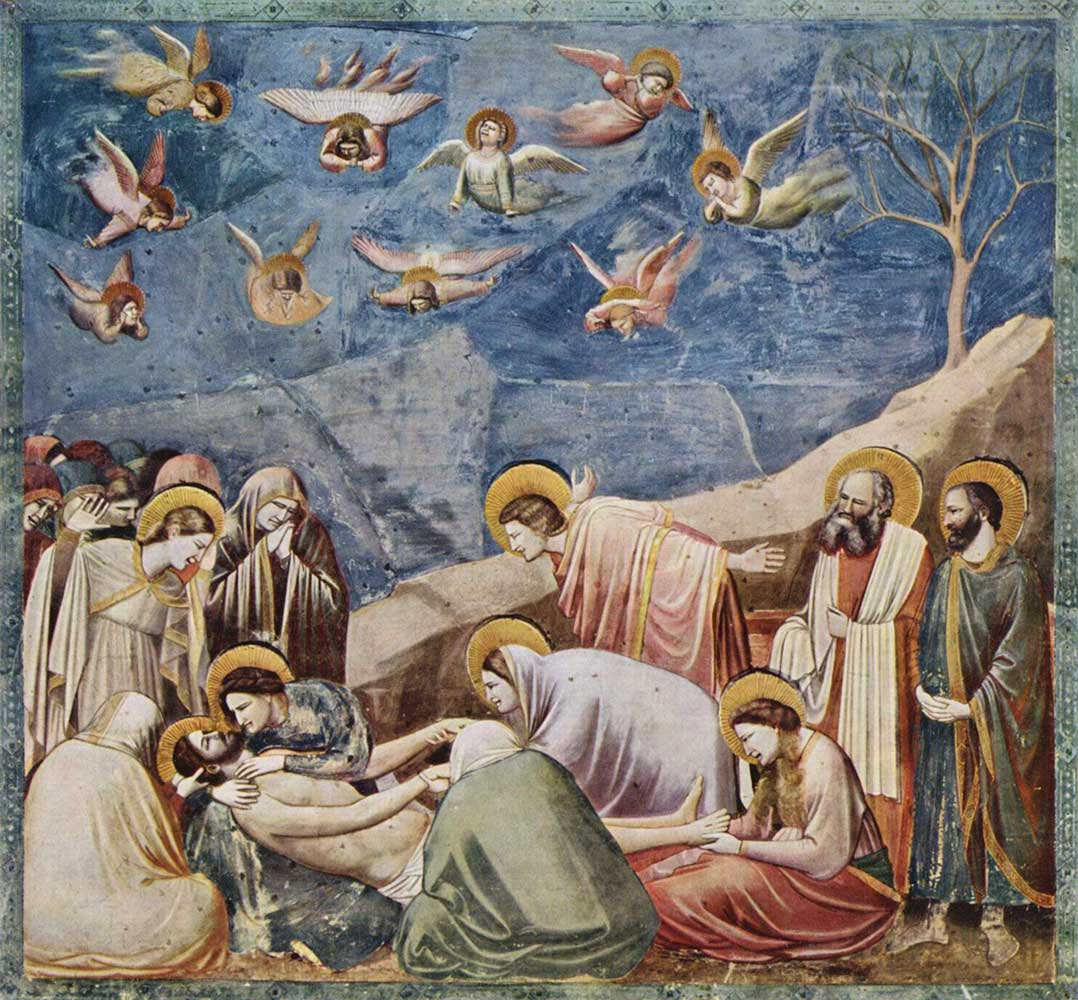
\includegraphics[width=0.8\textwidth]{./04-figuras/giotto_lamentacao}
    \label{fig:giotto_lamentacao}
  \end{center}
  \vspace*{-0,9cm}
  \fonte{\citeonline{muga}}\\
\end{figure}


\citeonline{muga} relata que é a partir do renascimento que o paradigma da luz atributo dá lugar ao da luz efeito. Além disso, conclui que foi mergulhando na \textit{camara oscura} que vários pintores do barroco e do renascimento perseguiram uma representação realista da natureza. E que, graças à ela Leonardo da Vinci desenvolveu o método \textit{chiaroscuro} e o \textit{sfumato}, reforçando a tridimensionalidade e a profundidade da representação, evidenciando, assim, o efeito da luz incidente e das partículas atmosféricas na difusão da luz. Esse estudo,  como podemos ver na figura \ref{fig:da_vinci_virgem_rochedos}, \textit{A virgem dos rochedos} de Leonardo da Vinci, é desenvolvido no seio da escuridão que antes atributo do mal, torna-se aliada para se chegar à luz, afirma \citeonline{muga}.

\begin{figure}[H]
  \begin{center}
    \caption{\textit{A virgem dos rochedos} (1495-1508), Leonardo da Vinci}
    \vspace*{0,2cm}
    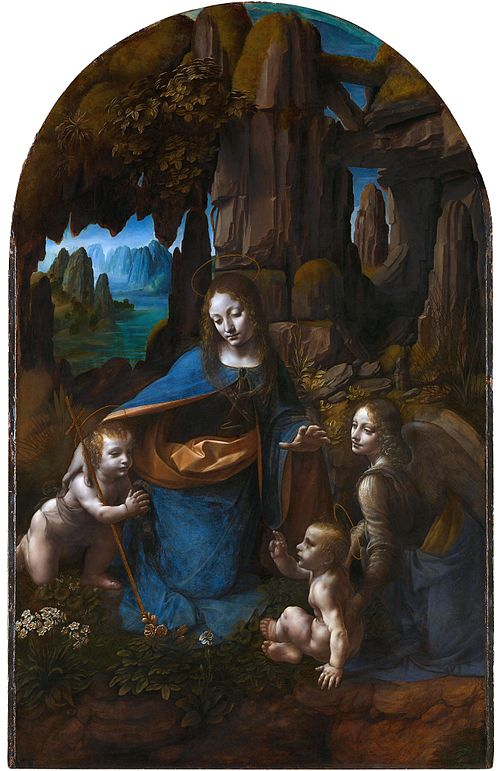
\includegraphics[width=0.4\textwidth]{./04-figuras/da_vinci_virgem_rochedos}
    \label{fig:da_vinci_virgem_rochedos}
  \end{center}
  \vspace*{-0,9cm}
  \fonte{\citeonline{muga}}\\
\end{figure}

Com o advento da fotografia os pintores precisaram se reinventar. Para \citeonline[p. 77]{henno} "o progresso tecnológico atrelado a fotografia exigiu que os artistas deslocassem o hábito descritivo da mimesis para um desenvolvimento interno de sua criatividade". Voltando a \citeonline{muga}, a fotografia influenciou os impressionistas a saírem do ateliês e procurarem no interior do globo ocular a percepção de uma natureza que, a cada mutação de luz, mudava de aspecto e de verdade. Segundo \apudonline{gombrich}{muga} Édouard Manet e seus seguidores descobriram que "ao olharmos a natureza ao ar livre e à plena luz do dia, as formas redondas parecem planas, e não vemos os objetos cada um com a sua cor própria, mas uma mistura brilhante de matizes que se combinam nos nossos olhos".


De acordo com \citeonline[p. 78]{henno} foi apoiado no preceito de que a cor se mistura no olho e não na paleta que Seurat aplicava pontos de cor na tela, em locais estratégicos, a fim de que a mistura desses pontos, a partir de uma distância apropriada, fossem vistos como uma única cor pelo observador. Na figura \ref{fig:seurat_la_parede} podemos ver a obra  \textit{La Parede} do artista e na figura \ref{fig:seurat_la_parede_detalhe} um detalhe ampliado desta mesma obra, que nos faz perceber como a mesma é constituída.


\begin{figure}[H]
  \begin{center}
    \caption{\textit{La Parade} (1887-88), Georges Seurat}
    \vspace*{0,2cm}
    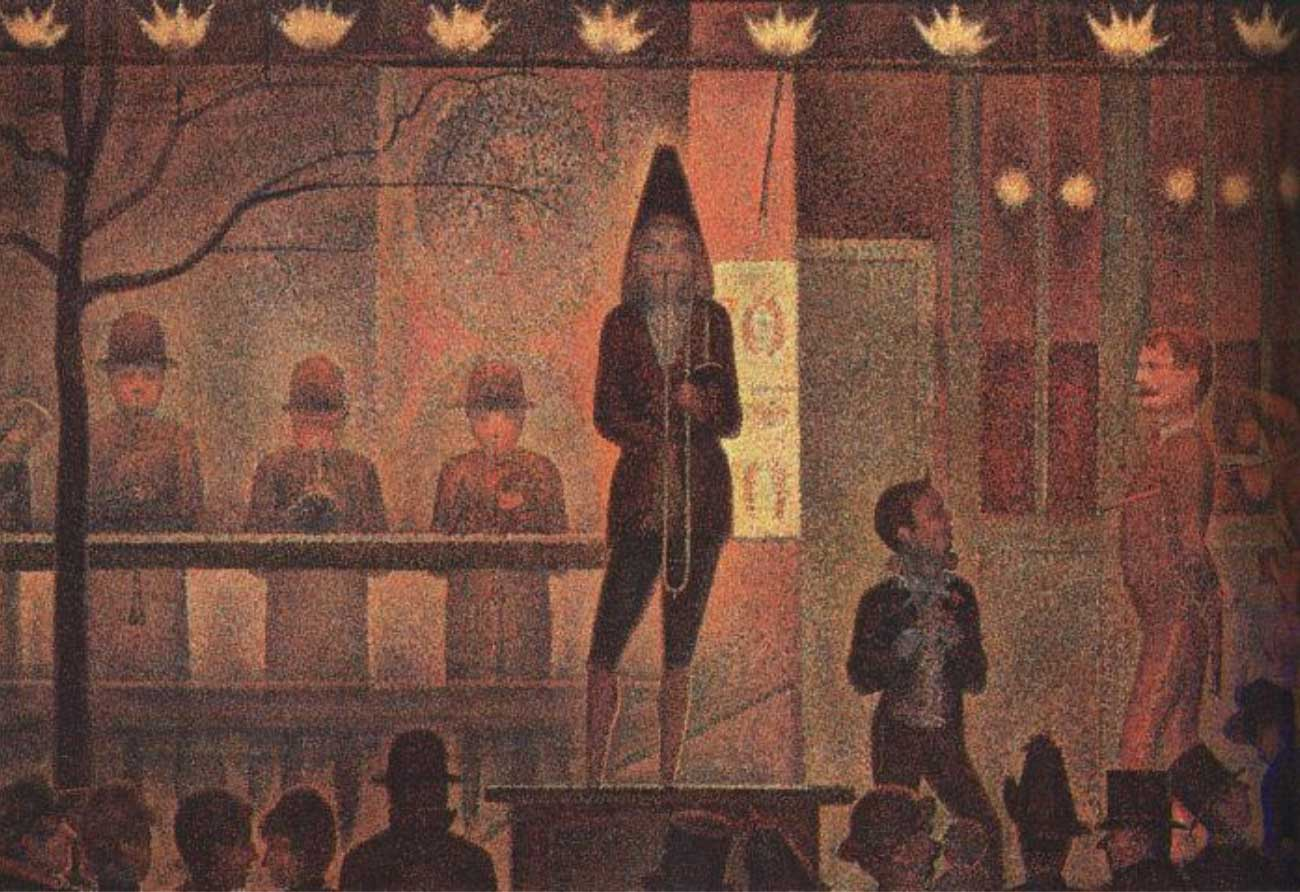
\includegraphics[width=0.8\textwidth]{./04-figuras/seurat_la_parede}
    \label{fig:seurat_la_parede}
  \end{center}
  \vspace*{-0,9cm}
  \fonte{\citeonline[p.79]{henno}}\\
\end{figure}

\begin{figure}[H]
  \begin{center}
    \caption{\textit{La Parade} (1887-88) - detalhe ampliado, Georges Seurat}
    \vspace*{0,2cm}
    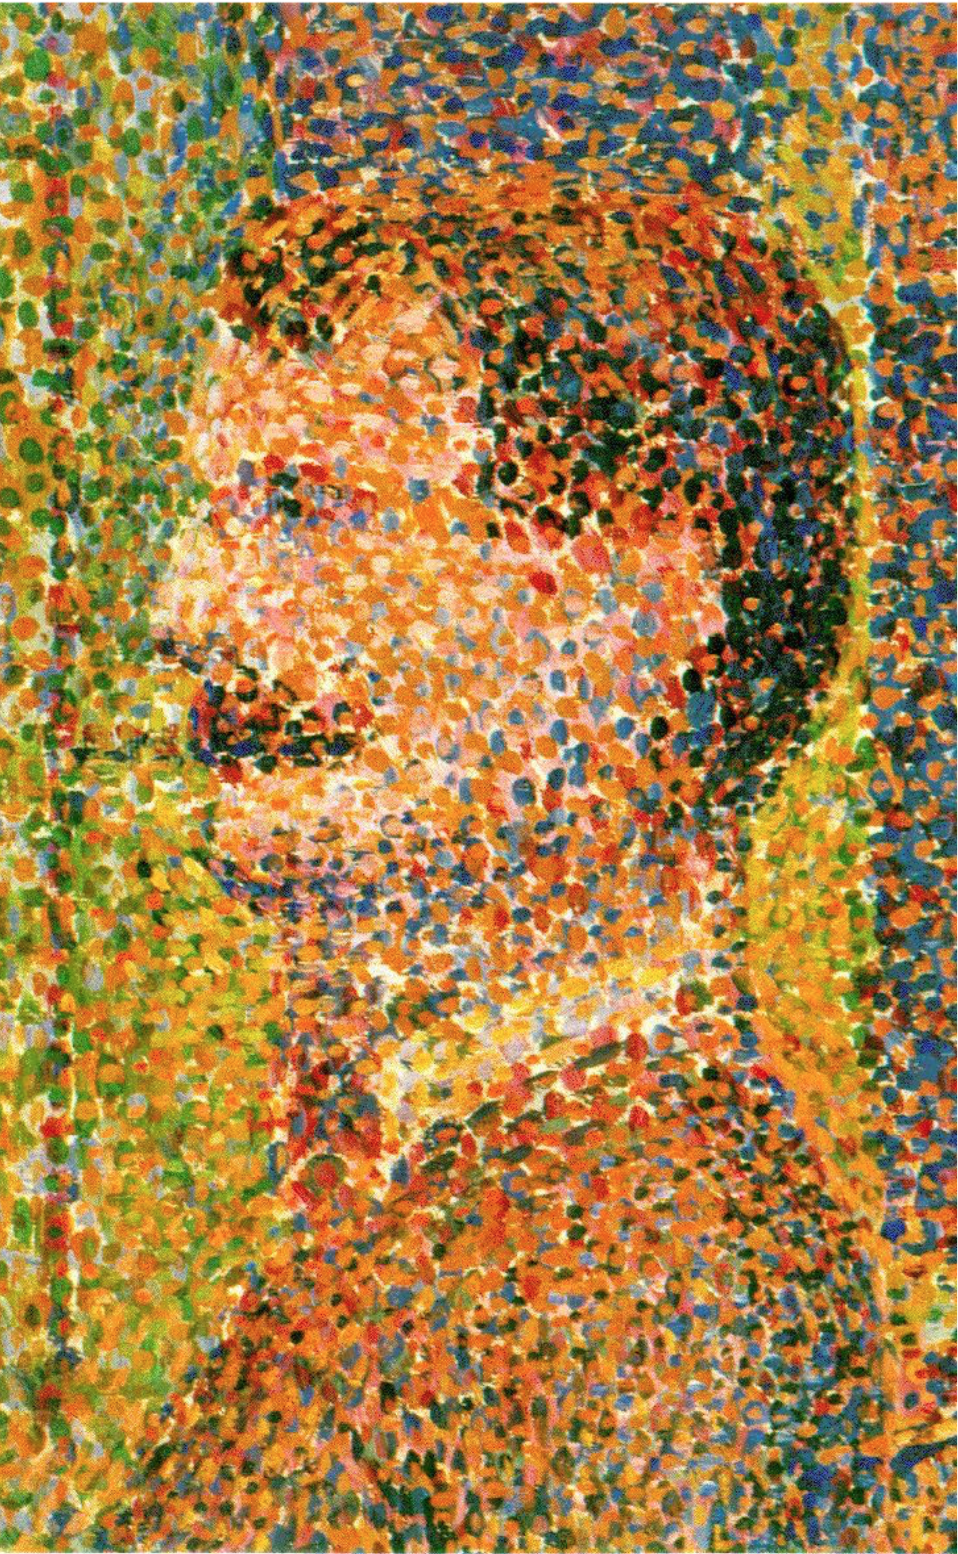
\includegraphics[width=0.4\textwidth]{./04-figuras/seurat_la_parede_detalhe}
    \label{fig:seurat_la_parede_detalhe}
  \end{center}
  \vspace*{-0,9cm}
  \fonte{\citeonline[p.79]{henno}}\\
\end{figure}


Para \citeonline{muga}, depois de ocupar o lugar de atributo brilhante e de efeito de iluminação, ao longo so século XX, a luz se torna um meio. Segundo \citeonline[p. 1]{azevedo} a função da luz não é mais somente de iluminar, de tornar visível uma obra ou um objeto, ou o mero reflexo dos seus efeitos suspensos no espaço. A luz passa a ser tratada como objeto ou material. Na perspectiva da arte contemporânea, se vê que, em muitas obras, a luz passa à matéria. \citeonline[p. 23]{vega} afirma que, atualmente, muitos artistas exploram as possibilidades da luz artificial, trabalhando com mescla de materiais e diversos tipos de fontes de luz. \citeonline[p. 50]{brandi} destaca que "alguns artistas e movimentos estéticos estão fortemente relacionados com a linguagem da luz, mesmo quando não a utilizam como objeto central da obra". 


James Turrell, por exemplo, foi pioneiro de uma nova preocupação com os fenômenos do espaço e da luz. Em seus primeiros trabalhos investigou os efeitos da luz artificial. Ele também desenvolveu várias instalações que aumentaram a relação entre a luz e a estrutura arquitetônica. Em conversa com \citeonline[p. 114]{adcock}, ele relata que uma das dificuldades de usar a luz é que ainda não é tradição utilizá-la em nossa cultura. Por outro lado, não é mais incomum usá-la do que usar pedra, argila, aço ou tinta. O artista declara seu interesse em trabalhar a luz como material, mas não luz em vidro, fibra de vidro ou acrílico, e sim no próprio espaço e nas qualidades do espaço, fazendo luz sem a forma física tradicional. Ele nos traz também que há uma rica tradição na pintura do trabalho sobre a luz, mas que isso de fato não é luz - é o registro da visão. Na figura \ref{fig:james_turrell} podemos ver sua obra entitulada \textit{The light inside} que transforma as paredes de um túnel em vasos para a condução da luz e nos dá uma ideia da dimensão na qual o artista trabalha este material. 

\begin{figure}[H]
  \begin{center}
    \caption{\textit{The light inside} (1999), James Turrell}
    \vspace*{0,2cm}
    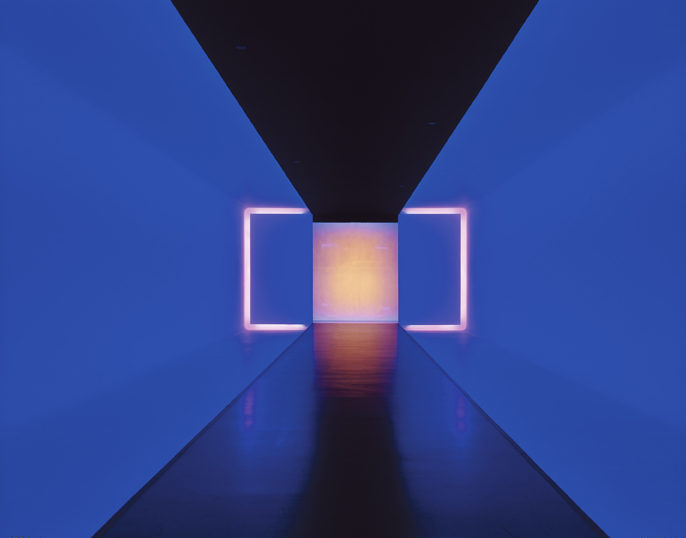
\includegraphics[width=0.8\textwidth]{./04-figuras/james_turrell}
    \label{fig:james_turrell}
  \end{center}
  \vspace*{-0,9cm}
  \fonte{Disponível em: <http://jamesturrell.com/work/thelightinside/>. \\ Acesso em: 18 jun. 2018}\\
\end{figure}

Já o trabalho de Jim Campbell chama à atenção pela antítese presente em suas obras. Em um vídeo produzido pela \citeonline{kqed}, o artista constata que em um mundo de alta definição e telas cada vez mais finas usa tecnologia para produzir o contrário: imagens borradas e em baixa resolução em painéis tridimensionais. Não há projeção. Essas vídeo-esculturas (figura \ref{fig:jim_campbell}) são compostas por grades de LEDs que atuam como uma televisão de pixels desconstruída. De perto, as luzes piscam de maneira desordenada, sendo apenas uma constelação de pontos brilhantes sem muito significado. A peça só começa a se revelar quando o espectador se afasta, tornando-se primeiro uma onda sincronizada de luzes em movimento e depois se transformando em imagens de crianças brincando ou homens e mulheres caminhando. 

\begin{figure}[H]
  \begin{center}
    \caption{\textit{Light Topography Wave} (2014), Jim Campbell}
    \vspace*{0,2cm}
    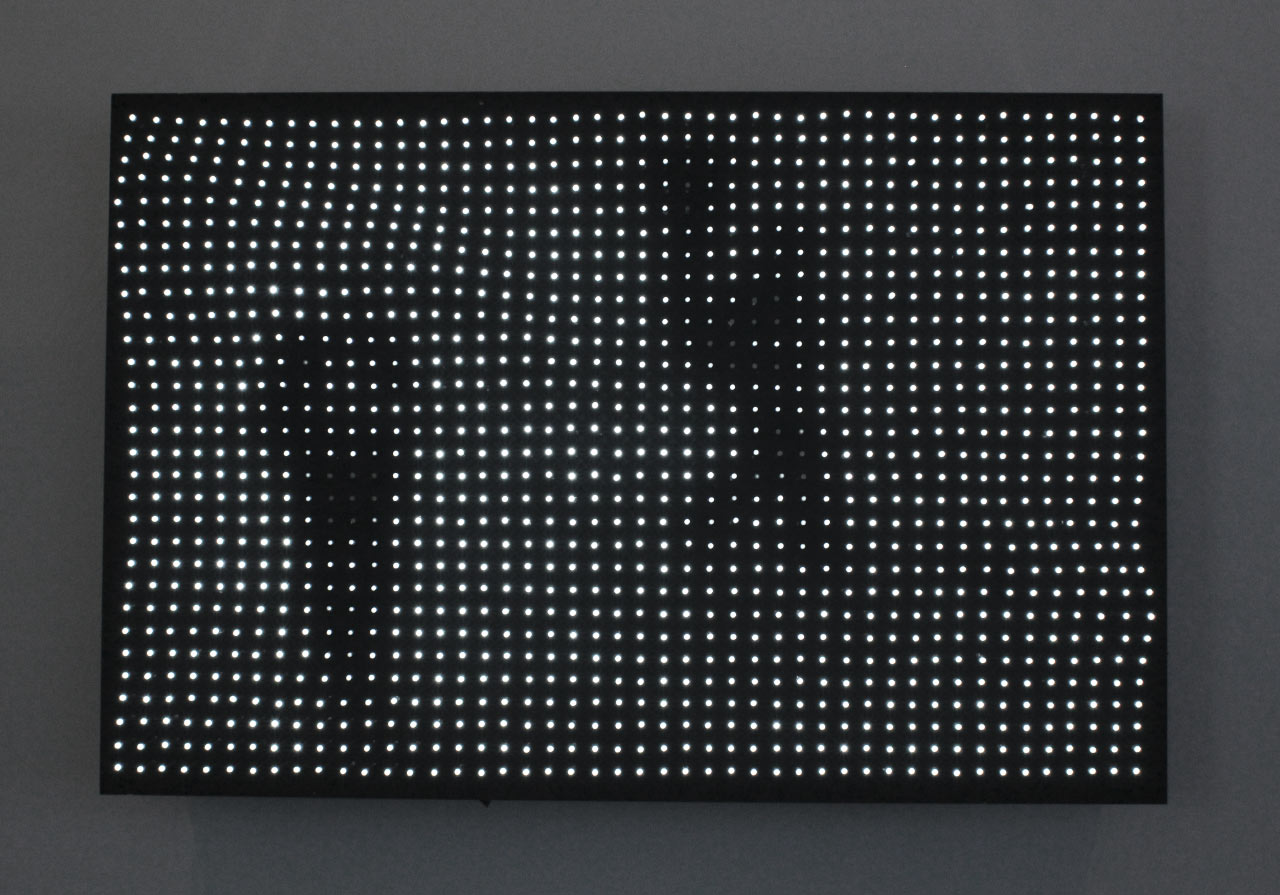
\includegraphics[width=0.8\textwidth]{./04-figuras/jim_campbell}
    \label{fig:jim_campbell}
  \end{center}
  \vspace*{-0,9cm}
  \fonte{Disponível em: <https://design-milk.com/pixelated-led-art-jim-campbell/>. \\ Acesso em: 22 mar. 2018}\\
\end{figure}


\section{LUZ E INTERATIVIDADE}

\citeonline[p. 73]{henno} afirma que, aliado ao desenvolvimento da ciência e da tecnologia, o homem de hoje tem condições de gerar e projetar a luz artificialmente ao invés de se restringir aos meios naturais. E que, ao se apropriar da luz, ele controla as emissões cromáticas a ela vinculadas, a partir de filtros ou de dispositivos tecnológicos específicos. Além disso, a autora relata que, atualmente, o artista dispõe de ferramentas que lhe possibilitam projetar através da luz. E, dessa forma, no caso da luz como fonte de emissão ou projeção, controla os dispositivos de luz, trabalhando poeticamente no momento em que confere um sentido à sua obra. Com o passar dos anos, os limites destes dispositivos se dissipam o que permite a interação homem e luz cada vez mais próxima. O reflexo dessa relação cada vez maior com os dispositivos técnicos, propicia uma abertura crescente da obra: o artista pode trabalhar em conjunto com o espectador na construção de seu sentido.


Um bom exemplo desta interação é a obra \textit{Optone} (figura \ref{fig:tsutomu_mutoh}), de autoria do designer Tsutomu Mutoh, que de acordo com \citeonline[p. 115]{henno}, usa um objeto com um eixo vertical que, em seu topo, possui uma cúpula contendo LEDs que se iluminam a partir do movimento aplicado pelo interator. Devido a seu peso e à ação da gravidade, a cúpula, pode ser movimentada sem que a base perca o contato com o solo. Assim, movimentos de rotação e balanço feitos por quem interage com o objeto são detectados por sensores, acionando os LEDs que estão dentro da cúpula. Ambos os dispositivos estão vinculados a um \textit{software}, desenvolvido pelo autor, que associa uma cor às coordenadas pelas quais a cúpula passa.

\begin{figure}[H]
  \begin{center}
    \caption{\textit{Optone} (2009), Tsutomu Mutoh}
    \vspace*{0,2cm}
    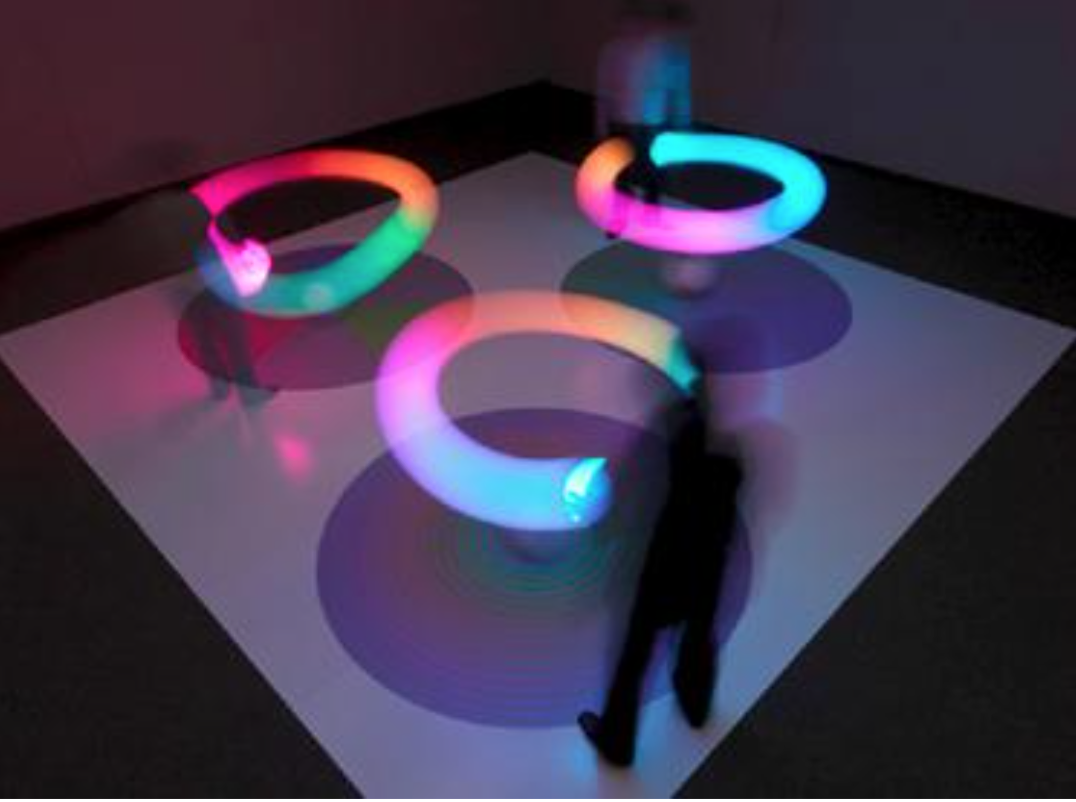
\includegraphics[width=0.8\textwidth]{./04-figuras/tsutomu_mutoh}
    \label{fig:tsutomu_mutoh}
  \end{center}
  \vspace*{-0,9cm}
  \fonte{\citeonline[p. 115]{henno}}
\end{figure}

Outro artista cuja obra é relevante no contexto deste trabalho e que, além da luz, explora a perspectiva da arte computacional, é o japonês Takahito Matsuo que, segundo \citeonline[p. 5]{soares}, cria mundos interativos de fantasia e de luz que fazem parte de uma estética enigmática, misturando som e luz perante os movimentos do observador. Seu trabalho destaca as diferentes gradações de luz e sombra que contrastando mostram um mundo de fantasia e imaginação. Em \textit{Fantasias Aquáticas Iluminadas} (figura \ref{fig:takahito_matsuo}), a exploração através de luz, projeções, arquitetura e interações humanas é fortemente encorajada. À medida que os visitantes se aproximam das paredes, se movimentam e se afastam, o número e a frequência das medusas aumentam e diminuem. As formas orgânicas e a brilhante paleta de azúis criam um mundo subaquático surreal, onde movimentos lúdicos e interações com o espaço arquitetônico resultam em uma comunicação não dita entre artista e participante. 

\begin{figure}[H]
  \begin{center}
    \caption{\textit{Fantasias Aquáticas Iluminadas} (2009), Takahito Matsuo}
    \vspace*{0,2cm}
    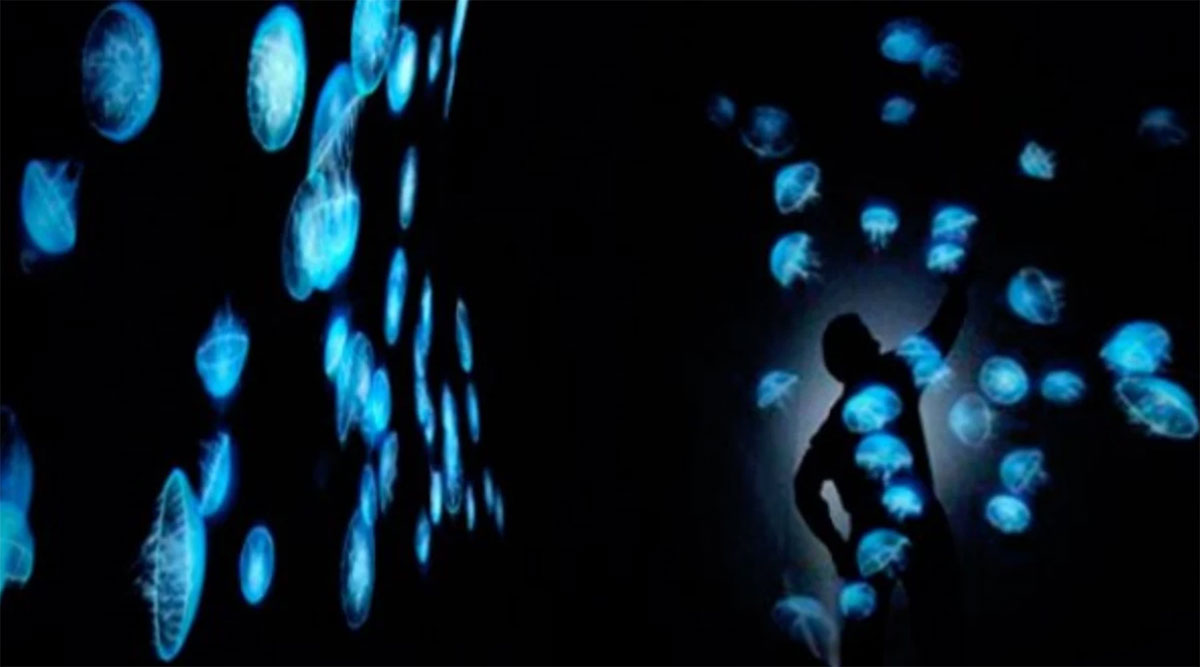
\includegraphics[width=0.8\textwidth]{./04-figuras/takahito_matsuo}
    \label{fig:takahito_matsuo}
  \end{center}
  \vspace*{-0,9cm}
  \fonte{\citeonline{soares}}
\end{figure}

\section{O CUBO PRETO}

O cubo branco tende a não ser o cenário ideal para exibição de obras que tem a luz como material. \citeonline[p. 40]{soares}, afirma que "a maioria dos autores que trabalham com arte e tecnologia procuram o espaço do cubo preto como espaço expositivo. Neste espaço o que interessa é um novo ver, um espanto com a imagem". Diz ainda que o nome cubo preto para este tipo de exposição surge em contraposição ao cubo branco, criado por Brian O'Doherty, num ensaio publicado pela revista Artforum em 1976, fazendo alusão ao espaço das galerias de arte, com paredes brancas, sem janelas isolando o espetador num meio aparentemente atemporal. A ideia do cubo preto surge como ambiente ideal para propagação da luz e é também uma forma de imersão no interior da mente do artista.

De acordo com \citeonline[p. 63]{sogabe2011} quando pensamos em instalações interativas, temos a lembrança de uma sala fechada e escura. Ele diz que essa condição está relacionada ao tipo de projetores de imagens existentes em uma época, com baixa luminosidade e que necessitavam de escuridão para apresentarem imagens nítidas. O autor afirma que, atualmente, essa condição já não é obrigatória, pois temos projetores de alta luminância, que podem funcionar em ambientes totalmente iluminados. Conclui então que, pela melhora dos equipamentos, o ambiente escuro passa a ser uma opção e não uma condição necessária. Ainda que isso possa ser verdade no que tange à imagem projetada, quando se trata da luz como fonte de emissão não se pode dizer o mesmo. \citeonline[p. 125]{henno} afirma que quando há pouca ou nenhuma luminosidade, a intensidade das cores é maior e mais perceptível devido ao contraste com a escuridão. E, além disso, o contraste da cor como informação luminosa em face da escuridão estabelece comunicação com o observador seduzindo-o pelos sentidos que tal cor suscita.

